\documentclass[11pt]{article}
\usepackage[utf8]{inputenc}
\usepackage[english, italian]{babel}
\usepackage{amsmath, amssymb, graphicx, hyperref}

\title{Test Avanzato per Spell Check}
\author{Un Utente Qualsiasi}
\date{\today}

\begin{document}

\maketitle

\begin{abstract}
Questo è un \textbf{abstract} per verificare che parole erratte vengano segnalate correttamente. 
Anche l'uso di parole inglesi sbagliate, come \emph{incorret}, dovrebbe essere identificato.
\end{abstract}

\tableofcontents

\section{Introduzione}
Benvenuti in questo documento di prova. Qui vedremo:
\begin{enumerate}
    \item Come \textit{funzionano} le verifiche ortografiche,
    \item Quali tipi di errori sono \underline{detectati} (es. parole non comuni come \emph{gluglup}),
    \item La gestione di formule come:
    \[
        \int_{a}^{b} f(x) dx = F(b) - F(a)
    \]
\end{enumerate}

\subsection{Test di formule}
Le formule matematiche non dovrebbero causare problemi:
\begin{align}
    E &= mc^2 \\
    a^2 + b^2 &= c^2 \quad \text{(Teorema di Pitagora)}
\end{align}
Errori nascosti dentro \texttt{inline math}: $x^y == 0$ è sbagliato.

\subsection{Parole comuni LaTeX}
Parole come \LaTeX, \texttt{documentclass}, \textbf{itemize} e simili devono essere ignorate.

\section{Test di figure e riferimenti}
Le immagini e i riferimenti devono essere ignorati:
\begin{figure}[h]
    \centering
    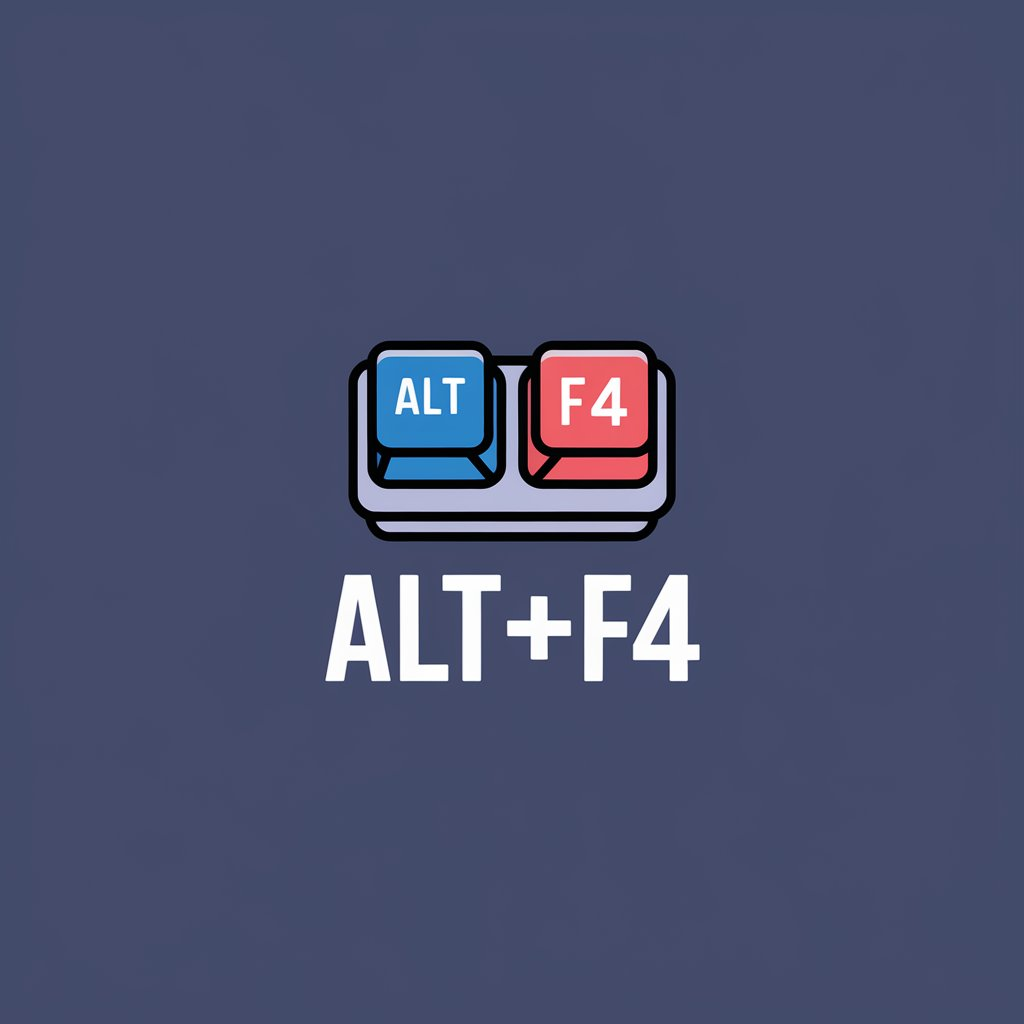
\includegraphics[width=0.5\textwidth]{Immagini/logo.jpeg}
    \caption{Una immagine di esempio.}
    \label{fig:example}
\end{figure}

Riferimento alla Figura~\ref{fig:example} è corretto, ma questo testo contine errori.

\section{Conclusioni}
Questo test include:
\begin{itemize}
    \item Errori in italiano: \emph{guistizia}, \textit{astrattoo},
    \item Errori in inglese: \emph{mistakess}, \textbf{grammer},
    \item Parole inventate: \texttt{qualikzze}, \texttt{pyrthonn}.
\end{itemize}

Per approfondire, visitare il sito ufficiale: \url{https://www.latex-project.org}.

\end{document}
